\documentclass[10pt,twocolumn,letterpaper]{article}


\usepackage{minted}
\usepackage{cvpr}
\usepackage{times}
\usepackage{epsfig}
\usepackage{graphicx}
\usepackage{caption}
\usepackage{subcaption}
\usepackage{dcolumn}
\usepackage{amsmath}
\usepackage{amssymb}
\usepackage{xcolor}
\definecolor{bg}{rgb}{0.95,0.95,0.95}


% Include other packages here, before hyperref.

% If you comment hyperref and then uncomment it, you should delete
% egpaper.aux before re-running latex.  (Or just hit 'q' on the first latex
% run, let it finish, and you should be clear).
\usepackage[breaklinks=true,bookmarks=false]{hyperref}

\cvprfinalcopy % *** Uncomment this line for the final submission

\def\cvprPaperID{****} % *** Enter the CVPR Paper ID here
\def\httilde{\mbox{\tt\raisebox{-.5ex}{\symbol{126}}}}

% Pages are numbered in submission mode, and unnumbered in camera-ready
%\ifcvprfinal\pagestyle{empty}\fi
\setcounter{page}{4321}
\begin{document}

%%%%%%%%% TITLE
\title{BSDS500 benchmark laboratory report}

\author{José Antonio Valero Medina\\
Universidad Distrital "Francisco José de Caldas"\\
Carrera 7 No. 40B - 53, Bogotá D.C. - República de Colombia\\
{\tt\small jvalero@udistrital.edu.co}
% For a paper whose authors are all at the same institution,
% omit the following lines up until the closing ``}''.
% Additional authors and addresses can be added with ``\and'',
% just like the second author.
% To save space, use either the email address or home page, not both
}

\maketitle
%\thispagestyle{empty}

%%%%%%%%% ABSTRACT
\begin{abstract}
   Here it is reported and discussed a segmentation algorithm adjust and evaluation based on Berkeley Segmentation Data Set and Benchmarks 500 (BSDS500). The first task was segmenting train images available on BSDS500, in order to adjust the own segmentation function produced in the segmentation laboratory (the previous one). After algorithm adjusting, the two methods were chosen and applied to the BSDS500 test images. The outcome images so obtained were evaluated against BSDS500 human ground truth versions using
   the methodology defined in BSDS500 benchmark. The own segmentation algorithm basically uses the facilities
   provided by mathlab software for each standard method (k-means, GMM, hierarchical grouping or watershed
   transform) used. As it was expected, the results were much less than optimums compared with the state-of-art
   as can be seen on the figures in the following.
\end{abstract}

%%%%%%%%% BODY TEXT
\section{Introduction}

Here it is reported and discussed a segmentation algorithm adjust and evaluation based on Berkeley Segmentation
Data Set and Benchmarks 500 (BSDS500). The work done as part of the BSBS500 laboratory started with \textit{segment\_by\_clustering} segmentation algorithm produced during the previous laboratory. This algorithm had been implemented for an image and a number of cluster given (beside of a method and a feature space). Then, it was necessary to implement it in a way that outcome segmentation images could be used in the BSDS500 benchmark. This means the segmentation algorithm should be able to create a segmentation hierarchy from which it was possible to produce several segmentation images each one with different number of clusters.

Two segmentation method were used.One was the hierarchical clustering which start considering each pixel as a group; next, in an iterative process, each group is merged with the nearest one using some distance measurement as a nearness criteria. The other one method was watershed transformation which, treating to an image as a surface, starts finding and less-to-greater sorting all the local minimums for next, by a flooding algorithm, tracing the watershed of each basin. The final watershed stage consists in merge the obtained basins in a way that is possible to create a segmentation hierarchy using a hierarchical grouping (in the case here discussed).

Those methods were used because of their advantageous hierarchical process which has to be run only once and then used to produce all of necessary segmentation images with any number of clusters. This contrasts with k-means and GMM methods which must be run once for each number of cluster as they do not create segmentation hierarchies. The feature space \textit{Lab} was used for representing the color space as this is an uniform color space, so the magnitude of differences in coordinates are good indicators of color distance doing them more perceptually meaningful \cite{Szeliski2010}.

The chosen feature space and methods were applied to the BSDS500 databases first to a small one, in a training stage for adjusting the algorithm, and then to the biggest available, for testing and evaluating it. The evaluation outcomes showed, as it was expected, the algorithm produces segmentation images which are less than optimums compared with the state-of-art as can be seen on the figures in the following. That is because of the algorithm basically uses the facilities provided by \textit{mathlab} software for each standard method (k-means, GMM, hierarchical grouping or watershed transform) used.

It is clear that methods implemented in the own algorithm can be improved by including additional descriptors as the use of oriented texture gradients or patch patterns drawn by humans as state-of-art has proposed. But, it is also possible to think in getting a hand of multispectral images where the same object differently responses in different wave lengths, e.g. doing possible discriminate alive and not alive objects in the thermal infrared in a clothes invariant way.

%-------------------------------------------------------------------------
\section{Data and methods}

BSDS500 test images were used in evaluating outcomes of the own segmentation algorithm, which was already implemented in the previous laboratory. This database is composed of two hundred realistic natural images which were segmented and labeled by humans. Each one image is about of four hundred rows and columns length, original images are in the \textit{rgd} feature space stored in \textit{jpg} format. The human segmentation images (five versions for each one) are \textit{matlab structure cell} variables saved on disk as \textit{.mat} files. Human labeling and segmenting are taken as the ground truth.

The database is organized as two big datasets, one for human segmentation images (the ground truth) and the other one for the original images, whit three stages: train, test and evaluation. The segmentation outcomes obtained from any algorithm applying can be saved as a \textit{.mat} file that contains a cell array containing several matrices which represent different segmentation scales.

First activity was to adjust the own algorithm interface since it had been implemented for being run for only one image, feature space, grouping method and number of clusters value set. Hierarchical and watershed grouping methods was chosen for this laboratory as they produce, running them only once, a segmentation hierarchy from which it is possible to obtain any necessary number of cluster in contrasting with k-means and GMM methods which must be run once for each number of cluster.

In \textit{watershed} method, for gradient calculating a single channel image was computed from a averaged sum of input channels as is shown in the following \textit{matlab} function snip:

\begin{minted}[bgcolor=bg]{matlab}
                 	...
                	
for i = 1:nchanels,
 singleChannel = singleChannel + ...
  double(downSampImage(:,:,i)) / ...
  double(nchanels);
end

Iy = imfilter(double(singleChannel), ...
 hy, 'replicate');
Ix = imfilter(double(singleChannel), ...
 hx, 'replicate');
totalGradient = sqrt(Ix.^2 + Iy.^2);
basins = watershed(totalGradient);
                    
                    ...
\end{minted}


For \textit{watershed} method the segmentation hierarchy was produced in an iterative grouping with extended minima as markers as indicated by the following code snip:

\begin{minted}[bgcolor=bg]{matlab}
			...
			
for h = 10:10:100,
 marker = imextendedmin(tGradient, ...
  h);
 new_grad = imimposemin(tGradient, ...
  marker);
 basins = watershed(new_grad);
 basinsMedian = ordfilt2(basins,9, ...
  ones(3,3)); 
 basins(find(basins == 0)) = ...
  basinsMedian(find(basins == 0));
 imageSegs{h / 10} = ...
  imresize(reshape(basins,rows, ...
  cols), [initRows initCols], ...
  'nearest');
end
            
            ...
\end{minted}


For \textit{hierarchical} method, segmentation images was easily produced iterating on the segmentation hierarchy \textit{dataLinkage} obtained from the previous hierarchical grouping stage which is shown in the following \textit{matlab} function snip:

\begin{figure*}
    \centering
    \begin{subfigure}[b]{0.2\textwidth}
        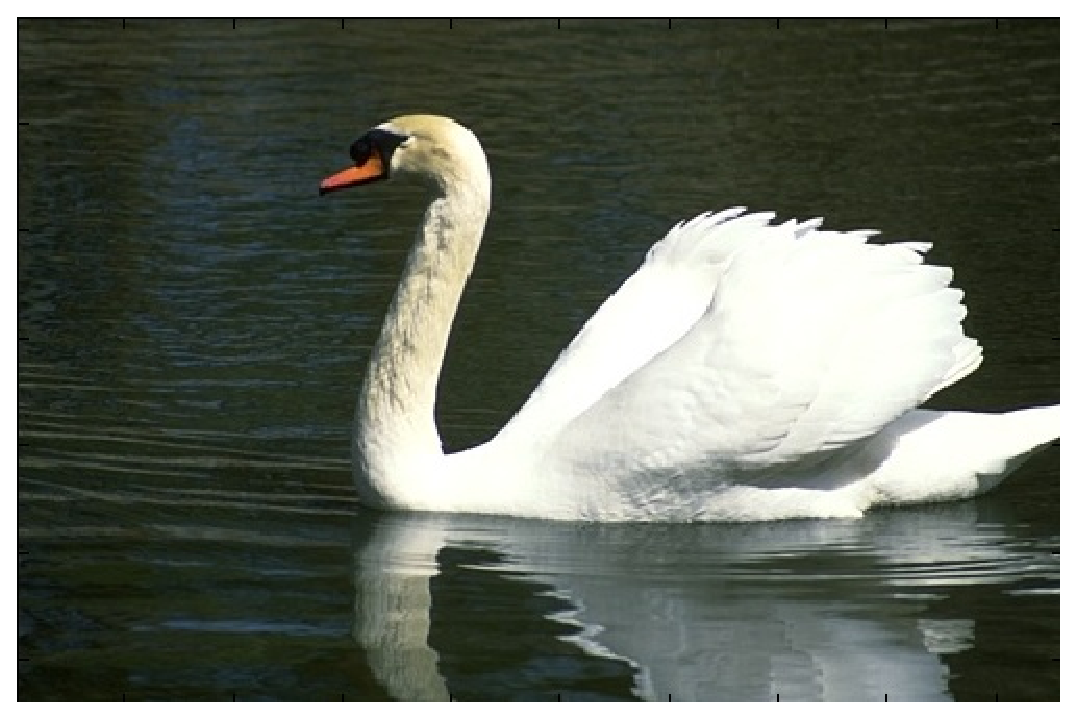
\includegraphics[width=\textwidth]{8068.eps}
        \caption{original}
    \end{subfigure}
    ~ 
    \begin{subfigure}[b]{0.2\textwidth}
        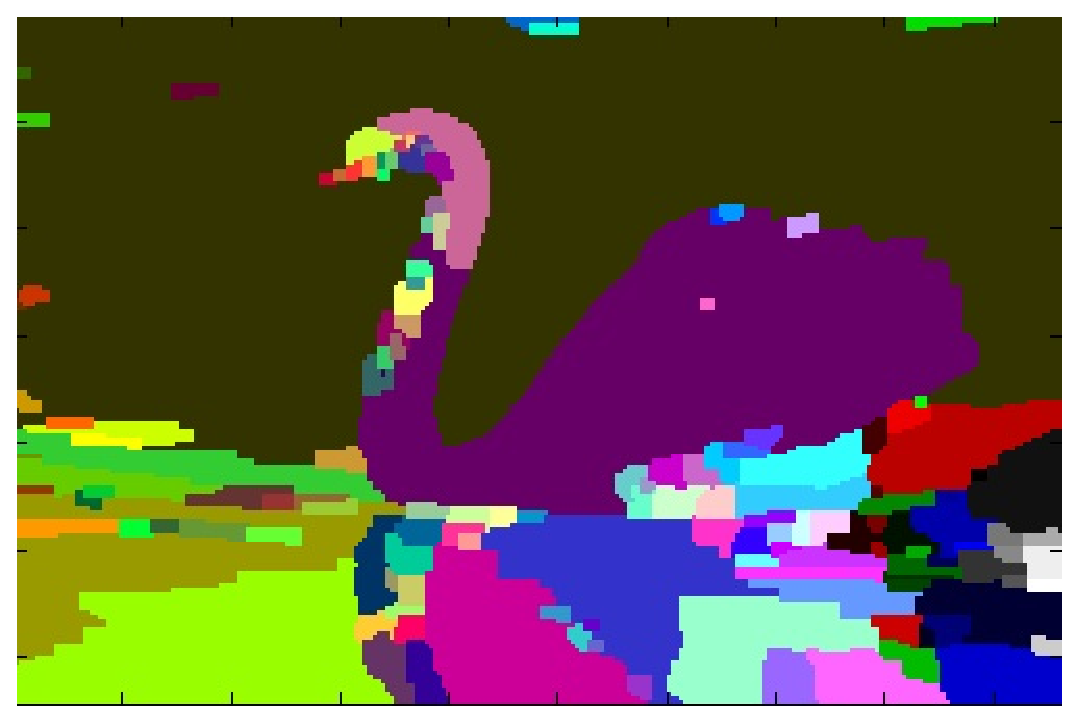
\includegraphics[width=\textwidth]{8068Wath10.eps}
        \caption{h = 10}
    \end{subfigure}
    ~ 
    \begin{subfigure}[b]{0.2\textwidth}
        
\includegraphics[width=\textwidth]{8068Wath30.eps}
        \caption{h = 50}
        \label{fig:h50}
    \end{subfigure}
    ~ 
    \begin{subfigure}[b]{0.2\textwidth}
        
\includegraphics[width=\textwidth]{8068Wath70.eps}
        \caption{h = 70}
    \end{subfigure}
   \caption{Segmentation hierarchy images got after applying a watershed grouping  with extended minima as markers.}
   \label{fig:watershed}
\end{figure*}

\begin{figure*}
    \centering
    \begin{subfigure}[b]{0.2\textwidth}
        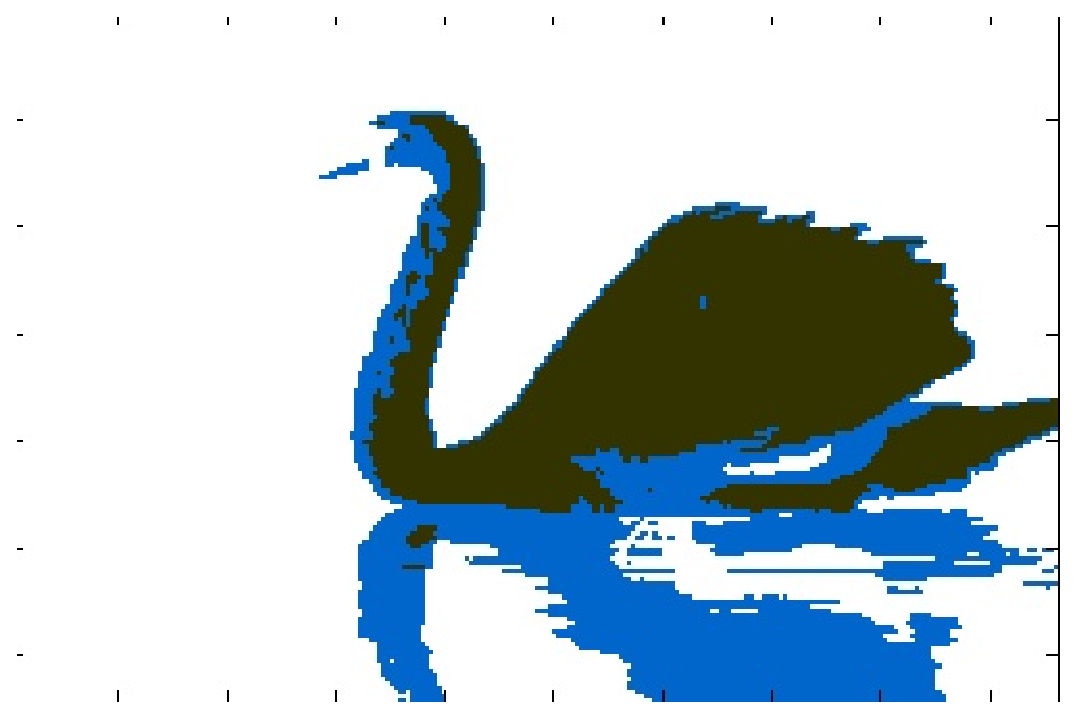
\includegraphics[width=\textwidth]{8068Hier3.eps}
        \caption{3 clusters}
        \label{fig:clust3}
    \end{subfigure}
    ~ 
    \begin{subfigure}[b]{0.2\textwidth}
        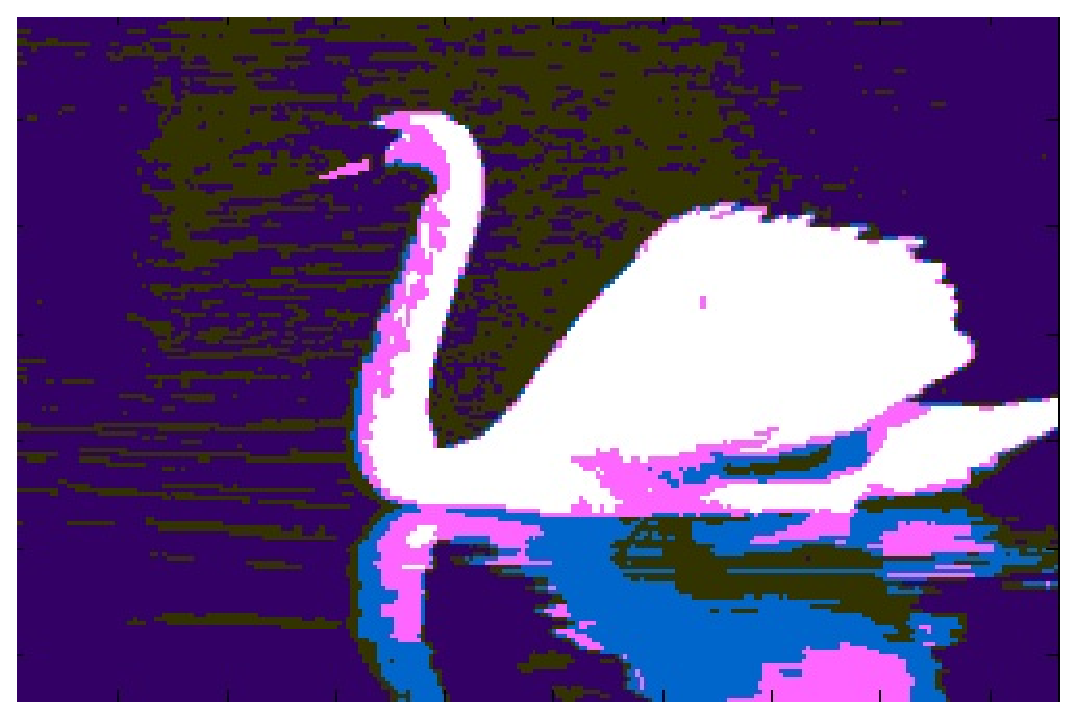
\includegraphics[width=\textwidth]{8068Hier5.eps}
        \caption{5 clusters}
        \label{fig:clust5}
    \end{subfigure}
    ~ 
    \begin{subfigure}[b]{0.2\textwidth}
        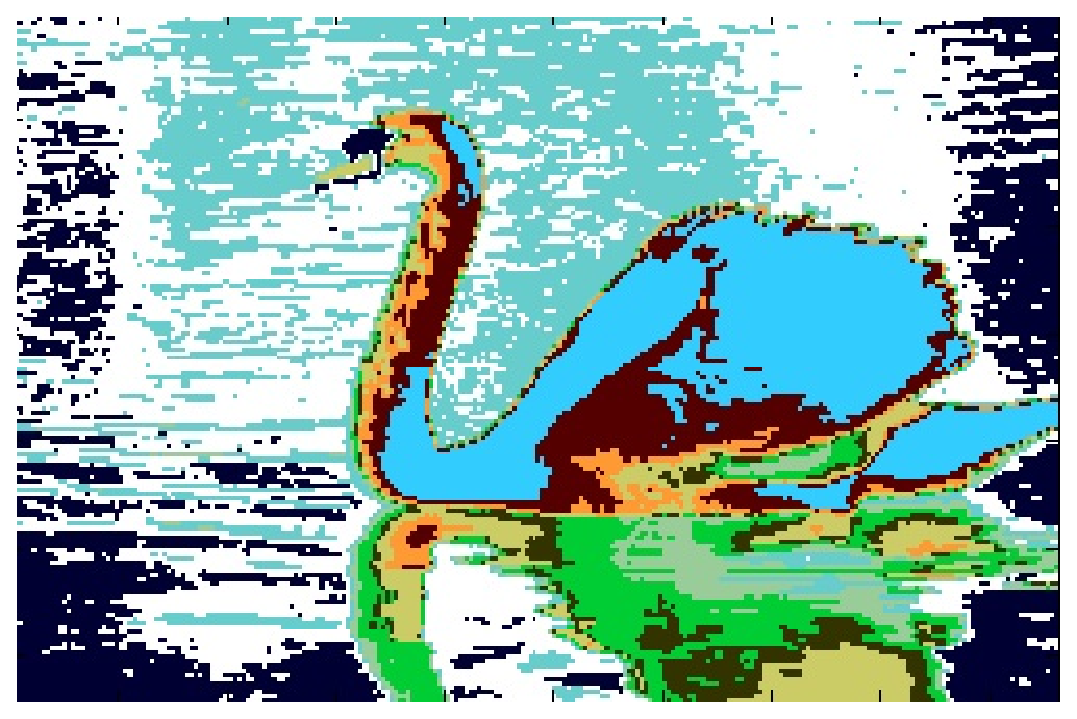
\includegraphics[width=\textwidth]{8068Hier10.eps}
        \caption{10 clusters}
        \label{fig:clust10}
    \end{subfigure}
    ~ 
    \begin{subfigure}[b]{0.2\textwidth}
        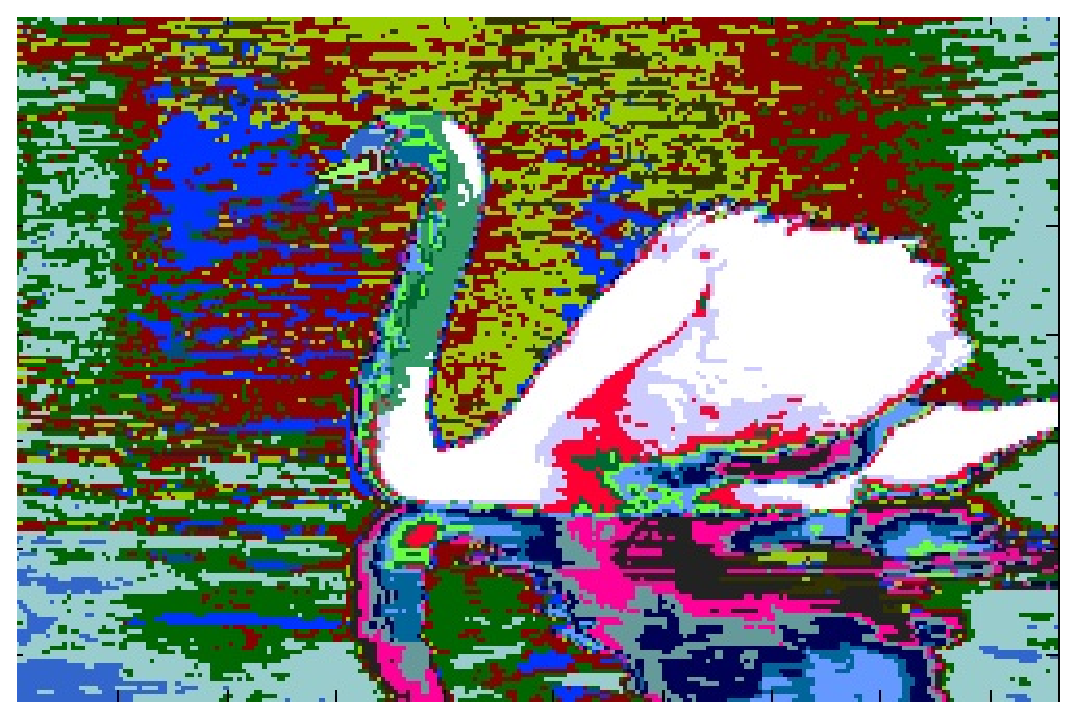
\includegraphics[width=\textwidth]{8068Hier20.eps}
        \caption{20 clusters}
        \label{fig:clust20}
    \end{subfigure}
   \caption{Segmentation hierarchy images got after applying a hierarchical grouping.}
   \label{fig:hierarchy}
\end{figure*}

\begin{minted}[bgcolor=bg]{matlab}
case {'hierarchical','watershed'},
		...            
            
for i = 1:size(clusterRange,2),
 cluster_idx = cluster(dataLinkage, ...
  'maxclust',clusterRange(i));
 imageSegs{i} = ...
  imresize(reshape(cluster_idx,rows, ...
  cols), [initRows initCols], 'nearest');
end
            
            ...
\end{minted}


Five training original and ground truth images from BSDS500 \textit{data} directory were used for adjusting the own algorithm parameter. A segmentation hierarchy was obtained for each image and method whit 99 cluster sizes going from two to one hundred. Each segmentation hierarchy had its precision-recall curve calculated using a \textit{bench\_bsds500} function modified version. After trying with training images, a test stage was conducted using the two hundred BSDS500 test images available in the \textit{BSDS500/data} directory. The benchmark evaluates the segmentation boundary and region precision and recall comparing each image of a segmentation hierarchy against each image version of the respective ground truth test image dataset. Since the boundary contour lines are not produced during the grouping stage, the benchmark framework calculates them directly from the segmentation images.


\section{Results}
 
First, the benchmark was successfully run on ten segmented images produced for each one of five initial training dataset images using watershed method. Figure~\ref{fig:watershed} shows  an example in which, beside the original image, the segmented images for different h values are shown.

Next, the benchmark was run on 99 segmented images produced by using the hierarchical grouping method. Figure~\ref{fig:hierarchy} shows a subset of the segmentation hierarchy obtained for three, five, ten and twelve number of clusters. As can be seen, the larger is the number of clusters better is the recall indicator because more (little) clusters have 100\% of coverage but the precision one gets badder as the false positives are so much. Therefore, the number of groups begins to be an obstacle to obtain good values of accuracy measures, the extent which it increases too above the number of objects in the human segmented image. 

The falling precision and increasing recall values tendency above mentioned can be verified by examining the evaluation outcomes for this two runs on Figure~\ref{fig:pFall_rRaise}. The red curve corresponds to \cite{Arbelaez2011} outcome which uses texture oriented gradient and pixel affinity additional stages in segmenting natural images. The green one is the outcome of P-R evaluation applied to the watershed segmentation method using only five training images. The blue one is the outcome of P-R evaluation  applied to the hierarchical segmentation method with a hundred segmented images using the same previous five training images. 

\begin{table*}
\begin{center}
\begin{subtable}{.5\textwidth}
\begin{center}
\begin{tabular}{|c|c|c|c|c|}
\hline
Method & ODS & th & 
OIS & Area\_PR \\
\hline\hline
ucm & F( 0.73, 0.73 ) = 0.73 & 0.13 & 
F( 0.77, 0.75 ) = 0.76 & 0.73\\
Watershed & F( 0.75, 0.56 ) = 0.64 & 2.16 & 
F( 0.69, 0.63 ) = 0.66 & 0.66\\
Hierarchical & F( 0.77, 0.50 ) = 0.61 & 2.00 &
F( 0.76, 0.51 ) = 0.61 & 0.18 \\
\hline
\end{tabular}
\caption{Boundary}
\end{center}
\end{subtable}
~
\begin{subtable}{.5\textwidth}
\begin{center}
\begin{tabular}{|c|c|c|c|c||c|c|c||c|c|c|}
\hline
\multicolumn{1}{|c|}{} &
\multicolumn{4}{c||}{GT covering} &
%\cline{2-4}
\multicolumn{3}{c||}{Rand Index} &
%\cline{5-7}
\multicolumn{3}{c|}{Var. Info.} \\
%\cline{8-10}
\hline
Method & ODS & th & OIS &  Best & 
ODS & th & OIS  & ODS & th & OIS \\
\hline\hline
ucm & 0.59 & 0.20 & 0.65 & 0.74 & 0.83 & 0.12 & 0.86 &
1.69 & 0.29 & 1.48 \\
Watershed & 0.53 & 2.00 & 0.61 & 0.68 & 0.82 & 2.00 & 0.87 &
2.00 & 4.00 & 1.89 \\
Hierarchical & 0.47 & 2.00 & 0.47 & 0.49 & 0.72 & 3.00 & 0.80 &
2.26 & 2.00 & 2.22 \\
\hline
\end{tabular}
\caption{Region}
\end{center}
\end{subtable}
\caption{Evaluation results for five training images.}
\label{tab:P_RT}
\end{center}
\end{table*}

Table~\ref{tab:P_RT} shows boundary quality measures for the training image set reporting the best F-measure on the dataset for a fixed scale (ODS) along with its threshold, the aggregate F-measure on the dataset for the best scale in each image (OIS) and the area under the precision-recall curve (Area\_PR). This table also show region quality measures computed by using the Optimal Dataset Scale (ODS), the Optimal Image Scale (OIS) for  covering of the ground-truth (GT covering) including the Best possible (Best), Probabilistic Rand Index (Rand Index) and Variation of information (Var. Info.) along with their respective thresholds (th). All measures are shown as provided by the benchmark framework.

\begin{figure}
\begin{center}
   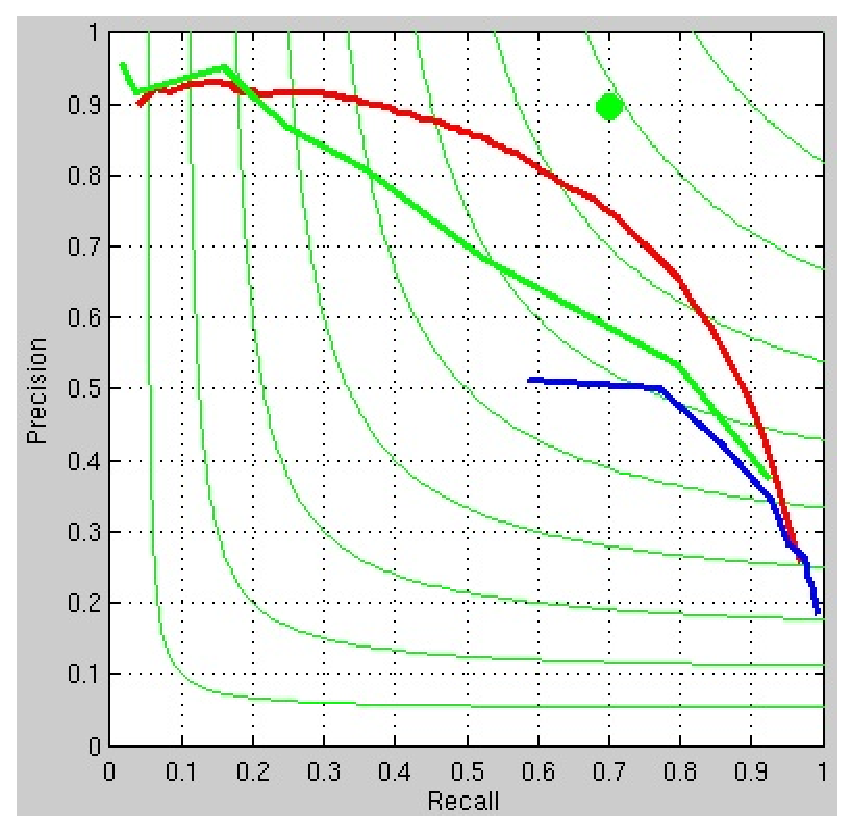
\includegraphics[width=0.8\linewidth]{pFall_rRaise.eps}
\end{center}
   \caption{P-R evaluation outcomes for different number of clusters and images.}
\label{fig:pFall_rRaise}
\end{figure}

After adjusting the own algorithm with training dataset, this was run for both \textit{watershed} and \textit{hierarchical} grouping methods, after that each one of two hundred test images got two segmentation hierarchy built, one for each method. The number of segmented images in a watershed segmentation hierarchy was ten (for different \textit{h} minimum values between 10 and 100) while in a hierarchical one was twenty (for cluster number between 1 to 20). No smaller values of \textit{h} or larger group numbers were used because with that only the recall is improved. The effort was dedicated to improving precision.

Finally, the benchmark was run on that two segmentation hierarchy set obtaining the outcomes shown on Figure~\ref{fig:P_RF}. Although the precision declined in both methods and more dramatically to the \textit{watershed} method, the latter remained above. As in the training image set, Table~\ref{tab:P_RF} shows boundary and region quality measures for the test image set.

\begin{figure}[t]
\begin{center}
   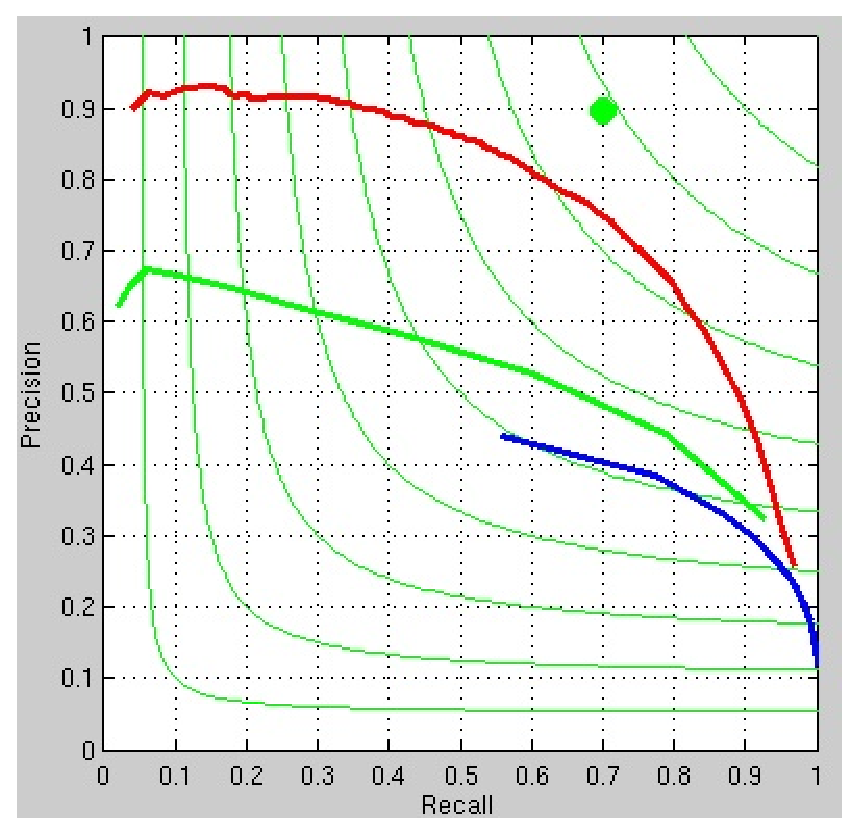
\includegraphics[width=0.8\linewidth]{P_RF.eps}
\end{center}
   \caption{P-R evaluation outcomes for 200 BSDS500 test images.}
\label{fig:P_RF}
\end{figure}

\begin{table*}
\begin{center}
\begin{subtable}{.5\textwidth}
\begin{center}
\begin{tabular}{|c|c|c|c|c|}
\hline
Method & ODS & th & 
OIS & Area\_PR \\
\hline\hline
ucm & F( 0.73, 0.73 ) = 0.73 & 0.13 & 
F( 0.77, 0.75 ) = 0.76 & 0.73\\
Watershed & F( 0.71, 0.48 ) = 0.57 & 2.42 & 
F( 0.74, 0.50 ) = 0.60 & 0.49\\
Hierarchical & F( 0.76, 0.39 ) = 0.51 & 2.96 &
F( 0.77, 0.42 ) = 0.55 & 0.28 \\
\hline
\end{tabular}
\caption{Boundary}
\end{center}
\end{subtable}
~
\begin{subtable}{.5\textwidth}
\begin{center}
\begin{tabular}{|c|c|c|c|c||c|c|c||c|c|c|}
\hline
\multicolumn{1}{|c|}{} &
\multicolumn{4}{c||}{GT covering} &
%\cline{2-4}
\multicolumn{3}{c||}{Rand Index} &
%\cline{5-7}
\multicolumn{3}{c|}{Var. Info.} \\
%\cline{8-10}
\hline
Method & ODS & th & OIS &  Best & 
ODS & th & OIS  & ODS & th & OIS \\
\hline\hline
ucm & 0.59 & 0.20 & 0.65 & 0.74 & 0.83 & 0.12 & 0.86 &
1.69 & 0.29 & 1.48 \\
Watershed & 0.45 & 3.00 & 0.51 & 0.60 & 0.78 & 2.00 & 0.81 &
2.43 & 5.00 & 2.10 \\
Hierarchical & 0.37 & 3.00 & 0.42 & 0.46 & 0.73 & 17.00 & 0.76 &
2.46 & 1.00 & 2.33 \\
\hline
\end{tabular}
\caption{Region}
\end{center}
\end{subtable}
\caption{Evaluation results for two hundred test images.}
\label{tab:P_RF}
\end{center}
\end{table*}

\section{Discussion}
After having adjusted the own algorithm it is clear that the information available directly on the feature space is not enough to get a good segmentation as the color similarity does not necessarily correspond with some geometric closeness.

That is the case of \textit{hierarchical} method when this was applied directly to a \textit{Lab} feature space producing geometrically disconnected segments as can be clearly seen in Figure~\ref{fig:clust3}, e.g. the black segment. It was thought that including the x (column) and y (row) pixel information as additional channels it could get better but it was not the case.

This situation became evident when comparing segmentations resulting, applying hierarchical grouping method, against segmentations performed by humans or against those got from owt-ucm method as can be seen on Table~\ref{tab:P_RT} and Table~\ref{tab:P_RF} for the really poor value of Area\_PR.

In contrast, the \textit{watershed} method has the advantage that while looking for local minimums in the feature space, this extends them to higher values in the same feature space  but looking at the pixels that are geometrically close to the pixels of those minimums. Now the sobel filtering stage was definitely necessary in order to set the higher values on borders. This effect can be noticed on Figure~\ref{fig:h50} where there is no disconnected region and the watershed boundaries match the swan borders.

The \textit{watershed} goodness is evident on Figure~\ref{fig:pFall_rRaise} where the respective PR curve, the green one, achieves high precision values in comparison with \textit{hierarchical}. Now, It is fair to clarify that this result was obtained with five training images but when more images are used, e.g. the test dataset, the precision measure goes dramatically down. This means that the watershed method here implemented is god for some images but not for all. The owt-ucm look a more general one.

\section{Improvements}
These results suggest that a good method of segmentation should not ignore watershed transform as this does merge very good the proximity concept of both geometric  and the feature spaces. In spite of that advantage, it is necessary to include other pixel descriptors in order to be more general as owt-ucm does.

It is clear that methods implemented in the own algorithm can be improved by including additional descriptors as the use of oriented texture gradients or patch patterns drawn by humans as state-of-art has proposed. But, it is also possible to think in getting a hand of multispectral images where the same object differently responses in different wave lengths, e.g. doing possible discriminate alive and not alive objects in the thermal infrared in a clothes invariant way.
%-------------------------------------------------------------------------


{\small
\bibliographystyle{ieee}
\bibliography{vision}
}

\end{document}
